% Options for packages loaded elsewhere
\PassOptionsToPackage{unicode}{hyperref}
\PassOptionsToPackage{hyphens}{url}
%
\documentclass[
]{article}
\usepackage{lmodern}
\usepackage{amssymb,amsmath}
\usepackage{ifxetex,ifluatex}
\ifnum 0\ifxetex 1\fi\ifluatex 1\fi=0 % if pdftex
  \usepackage[T1]{fontenc}
  \usepackage[utf8]{inputenc}
  \usepackage{textcomp} % provide euro and other symbols
\else % if luatex or xetex
  \usepackage{unicode-math}
  \defaultfontfeatures{Scale=MatchLowercase}
  \defaultfontfeatures[\rmfamily]{Ligatures=TeX,Scale=1}
\fi
% Use upquote if available, for straight quotes in verbatim environments
\IfFileExists{upquote.sty}{\usepackage{upquote}}{}
\IfFileExists{microtype.sty}{% use microtype if available
  \usepackage[]{microtype}
  \UseMicrotypeSet[protrusion]{basicmath} % disable protrusion for tt fonts
}{}
\makeatletter
\@ifundefined{KOMAClassName}{% if non-KOMA class
  \IfFileExists{parskip.sty}{%
    \usepackage{parskip}
  }{% else
    \setlength{\parindent}{0pt}
    \setlength{\parskip}{6pt plus 2pt minus 1pt}}
}{% if KOMA class
  \KOMAoptions{parskip=half}}
\makeatother
\usepackage{xcolor}
\IfFileExists{xurl.sty}{\usepackage{xurl}}{} % add URL line breaks if available
\IfFileExists{bookmark.sty}{\usepackage{bookmark}}{\usepackage{hyperref}}
\hypersetup{
  pdftitle={Militares por Raça},
  pdfauthor={Marcelo Ribeiro},
  hidelinks,
  pdfcreator={LaTeX via pandoc}}
\urlstyle{same} % disable monospaced font for URLs
\usepackage[margin=1in]{geometry}
\usepackage{color}
\usepackage{fancyvrb}
\newcommand{\VerbBar}{|}
\newcommand{\VERB}{\Verb[commandchars=\\\{\}]}
\DefineVerbatimEnvironment{Highlighting}{Verbatim}{commandchars=\\\{\}}
% Add ',fontsize=\small' for more characters per line
\usepackage{framed}
\definecolor{shadecolor}{RGB}{248,248,248}
\newenvironment{Shaded}{\begin{snugshade}}{\end{snugshade}}
\newcommand{\AlertTok}[1]{\textcolor[rgb]{0.94,0.16,0.16}{#1}}
\newcommand{\AnnotationTok}[1]{\textcolor[rgb]{0.56,0.35,0.01}{\textbf{\textit{#1}}}}
\newcommand{\AttributeTok}[1]{\textcolor[rgb]{0.77,0.63,0.00}{#1}}
\newcommand{\BaseNTok}[1]{\textcolor[rgb]{0.00,0.00,0.81}{#1}}
\newcommand{\BuiltInTok}[1]{#1}
\newcommand{\CharTok}[1]{\textcolor[rgb]{0.31,0.60,0.02}{#1}}
\newcommand{\CommentTok}[1]{\textcolor[rgb]{0.56,0.35,0.01}{\textit{#1}}}
\newcommand{\CommentVarTok}[1]{\textcolor[rgb]{0.56,0.35,0.01}{\textbf{\textit{#1}}}}
\newcommand{\ConstantTok}[1]{\textcolor[rgb]{0.00,0.00,0.00}{#1}}
\newcommand{\ControlFlowTok}[1]{\textcolor[rgb]{0.13,0.29,0.53}{\textbf{#1}}}
\newcommand{\DataTypeTok}[1]{\textcolor[rgb]{0.13,0.29,0.53}{#1}}
\newcommand{\DecValTok}[1]{\textcolor[rgb]{0.00,0.00,0.81}{#1}}
\newcommand{\DocumentationTok}[1]{\textcolor[rgb]{0.56,0.35,0.01}{\textbf{\textit{#1}}}}
\newcommand{\ErrorTok}[1]{\textcolor[rgb]{0.64,0.00,0.00}{\textbf{#1}}}
\newcommand{\ExtensionTok}[1]{#1}
\newcommand{\FloatTok}[1]{\textcolor[rgb]{0.00,0.00,0.81}{#1}}
\newcommand{\FunctionTok}[1]{\textcolor[rgb]{0.00,0.00,0.00}{#1}}
\newcommand{\ImportTok}[1]{#1}
\newcommand{\InformationTok}[1]{\textcolor[rgb]{0.56,0.35,0.01}{\textbf{\textit{#1}}}}
\newcommand{\KeywordTok}[1]{\textcolor[rgb]{0.13,0.29,0.53}{\textbf{#1}}}
\newcommand{\NormalTok}[1]{#1}
\newcommand{\OperatorTok}[1]{\textcolor[rgb]{0.81,0.36,0.00}{\textbf{#1}}}
\newcommand{\OtherTok}[1]{\textcolor[rgb]{0.56,0.35,0.01}{#1}}
\newcommand{\PreprocessorTok}[1]{\textcolor[rgb]{0.56,0.35,0.01}{\textit{#1}}}
\newcommand{\RegionMarkerTok}[1]{#1}
\newcommand{\SpecialCharTok}[1]{\textcolor[rgb]{0.00,0.00,0.00}{#1}}
\newcommand{\SpecialStringTok}[1]{\textcolor[rgb]{0.31,0.60,0.02}{#1}}
\newcommand{\StringTok}[1]{\textcolor[rgb]{0.31,0.60,0.02}{#1}}
\newcommand{\VariableTok}[1]{\textcolor[rgb]{0.00,0.00,0.00}{#1}}
\newcommand{\VerbatimStringTok}[1]{\textcolor[rgb]{0.31,0.60,0.02}{#1}}
\newcommand{\WarningTok}[1]{\textcolor[rgb]{0.56,0.35,0.01}{\textbf{\textit{#1}}}}
\usepackage{graphicx,grffile}
\makeatletter
\def\maxwidth{\ifdim\Gin@nat@width>\linewidth\linewidth\else\Gin@nat@width\fi}
\def\maxheight{\ifdim\Gin@nat@height>\textheight\textheight\else\Gin@nat@height\fi}
\makeatother
% Scale images if necessary, so that they will not overflow the page
% margins by default, and it is still possible to overwrite the defaults
% using explicit options in \includegraphics[width, height, ...]{}
\setkeys{Gin}{width=\maxwidth,height=\maxheight,keepaspectratio}
% Set default figure placement to htbp
\makeatletter
\def\fps@figure{htbp}
\makeatother
\setlength{\emergencystretch}{3em} % prevent overfull lines
\providecommand{\tightlist}{%
  \setlength{\itemsep}{0pt}\setlength{\parskip}{0pt}}
\setcounter{secnumdepth}{-\maxdimen} % remove section numbering

\title{Militares por Raça}
\author{Marcelo Ribeiro}
\date{08/12/2019}

\begin{document}
\maketitle

\begin{verbatim}
## Warning: package 'knitr' was built under R version 3.6.3
\end{verbatim}

\begin{verbatim}
## Warning: package 'rmdformats' was built under R version 3.6.3
\end{verbatim}

\begin{verbatim}
## Warning: package 'tidyverse' was built under R version 3.6.3
\end{verbatim}

\begin{verbatim}
## -- Attaching packages -------------------------------------------- tidyverse 1.3.0 --
\end{verbatim}

\begin{verbatim}
## v ggplot2 3.3.0     v purrr   0.3.3
## v tibble  2.1.3     v dplyr   0.8.5
## v tidyr   1.0.2     v stringr 1.4.0
## v readr   1.3.1     v forcats 0.5.0
\end{verbatim}

\begin{verbatim}
## Warning: package 'ggplot2' was built under R version 3.6.3
\end{verbatim}

\begin{verbatim}
## Warning: package 'tidyr' was built under R version 3.6.3
\end{verbatim}

\begin{verbatim}
## Warning: package 'purrr' was built under R version 3.6.3
\end{verbatim}

\begin{verbatim}
## Warning: package 'dplyr' was built under R version 3.6.3
\end{verbatim}

\begin{verbatim}
## Warning: package 'forcats' was built under R version 3.6.3
\end{verbatim}

\begin{verbatim}
## -- Conflicts ----------------------------------------------- tidyverse_conflicts() --
## x dplyr::filter() masks stats::filter()
## x dplyr::lag()    masks stats::lag()
\end{verbatim}

\begin{verbatim}
## 
## Attaching package: 'lubridate'
\end{verbatim}

\begin{verbatim}
## The following object is masked from 'package:base':
## 
##     date
\end{verbatim}

\begin{verbatim}
## Warning: package 'data.table' was built under R version 3.6.3
\end{verbatim}

\begin{verbatim}
## 
## Attaching package: 'data.table'
\end{verbatim}

\begin{verbatim}
## The following objects are masked from 'package:lubridate':
## 
##     hour, isoweek, mday, minute, month, quarter, second, wday, week,
##     yday, year
\end{verbatim}

\begin{verbatim}
## The following objects are masked from 'package:dplyr':
## 
##     between, first, last
\end{verbatim}

\begin{verbatim}
## The following object is masked from 'package:purrr':
## 
##     transpose
\end{verbatim}

\begin{verbatim}
## Warning: package 'e1071' was built under R version 3.6.3
\end{verbatim}

\begin{verbatim}
## Warning: package 'car' was built under R version 3.6.3
\end{verbatim}

\begin{verbatim}
## Loading required package: carData
\end{verbatim}

\begin{verbatim}
## 
## Attaching package: 'car'
\end{verbatim}

\begin{verbatim}
## The following object is masked from 'package:dplyr':
## 
##     recode
\end{verbatim}

\begin{verbatim}
## The following object is masked from 'package:purrr':
## 
##     some
\end{verbatim}

\begin{verbatim}
## Warning: package 'RcmdrMisc' was built under R version 3.6.3
\end{verbatim}

\begin{verbatim}
## Loading required package: sandwich
\end{verbatim}

\begin{verbatim}
## Warning: package 'survival' was built under R version 3.6.3
\end{verbatim}

\begin{verbatim}
## Warning: package 'ggfortify' was built under R version 3.6.3
\end{verbatim}

\begin{verbatim}
## Loading required package: gplots
\end{verbatim}

\begin{verbatim}
## Warning: package 'gplots' was built under R version 3.6.3
\end{verbatim}

\begin{verbatim}
## 
## Attaching package: 'gplots'
\end{verbatim}

\begin{verbatim}
## The following object is masked from 'package:stats':
## 
##     lowess
\end{verbatim}

\hypertarget{r-markdown}{%
\subsection{R Markdown}\label{r-markdown}}

Leitura dos dados

\begin{Shaded}
\begin{Highlighting}[]
\NormalTok{militares <-}\StringTok{ }\KeywordTok{read.csv2}\NormalTok{(}\StringTok{"militares.csv"}\NormalTok{)}
\end{Highlighting}
\end{Shaded}

Estatísticas descritivas

\begin{verbatim}
##      NR_REF      POSTO_GRADUACAO      QUADRO              RACA      
##  Min.   :    1   CB      :15527   QPPM   :33061   AMARELO   :  481  
##  1st Qu.: 9498   3 SGT   : 7069   QOPM   : 2028   BRANCO    :15698  
##  Median :18996   SD 1 CL : 6668   QPE    : 1119   INDIGENA  :  159  
##  Mean   :18996   2 SGT   : 3773   QOC    :  757   NAO INF.  :  871  
##  3rd Qu.:28494   2 TEN   : 1207   QOS    :  600   PARDO     :17869  
##  Max.   :37991   1 TEN   : 1017   QPEP   :  360   PRETO     : 2913  
##                  (Other) : 2730   (Other):   66
\end{verbatim}

Tabelas de contigências e teste qui quadrado para verificar associaçoes
entre as variaveis

\begin{Shaded}
\begin{Highlighting}[]
\KeywordTok{local}\NormalTok{(\{}
\NormalTok{    .Table <-}\StringTok{ }\KeywordTok{with}\NormalTok{(militares, }\KeywordTok{table}\NormalTok{(POSTO_GRADUACAO))}
    \KeywordTok{cat}\NormalTok{(}\StringTok{"}\CharTok{\textbackslash{}n}\StringTok{counts:}\CharTok{\textbackslash{}n}\StringTok{"}\NormalTok{)}
    \KeywordTok{print}\NormalTok{(.Table)}
    \KeywordTok{cat}\NormalTok{(}\StringTok{"}\CharTok{\textbackslash{}n}\StringTok{percentages:}\CharTok{\textbackslash{}n}\StringTok{"}\NormalTok{)}
    \KeywordTok{print}\NormalTok{(}\KeywordTok{round}\NormalTok{(}\DecValTok{100} \OperatorTok{*}\StringTok{ }\NormalTok{.Table}\OperatorTok{/}\KeywordTok{sum}\NormalTok{(.Table), }\DecValTok{2}\NormalTok{))}
\NormalTok{\})}
\end{Highlighting}
\end{Shaded}

\begin{verbatim}
## 
## counts:
## POSTO_GRADUACAO
## 1 SGT    1 TEN    2 SGT    2 TEN    3 SGT    ALUNO    ASP A OF CAD      
##      620     1017     3773     1207     7069       59        6      294 
## CAP      CB       CEL      MAJ      SD 1 CL  SD 2 CL  SUB TEN  TEN CEL  
##      563    15527       45      386     6668      121      404      232 
## 
## percentages:
## POSTO_GRADUACAO
## 1 SGT    1 TEN    2 SGT    2 TEN    3 SGT    ALUNO    ASP A OF CAD      
##     1.63     2.68     9.93     3.18    18.61     0.16     0.02     0.77 
## CAP      CB       CEL      MAJ      SD 1 CL  SD 2 CL  SUB TEN  TEN CEL  
##     1.48    40.87     0.12     1.02    17.55     0.32     1.06     0.61
\end{verbatim}

\begin{Shaded}
\begin{Highlighting}[]
\KeywordTok{local}\NormalTok{(\{}
\NormalTok{    .Table <-}\StringTok{ }\KeywordTok{with}\NormalTok{(militares, }\KeywordTok{table}\NormalTok{(QUADRO))}
    \KeywordTok{cat}\NormalTok{(}\StringTok{"}\CharTok{\textbackslash{}n}\StringTok{counts:}\CharTok{\textbackslash{}n}\StringTok{"}\NormalTok{)}
    \KeywordTok{print}\NormalTok{(.Table)}
    \KeywordTok{cat}\NormalTok{(}\StringTok{"}\CharTok{\textbackslash{}n}\StringTok{percentages:}\CharTok{\textbackslash{}n}\StringTok{"}\NormalTok{)}
    \KeywordTok{print}\NormalTok{(}\KeywordTok{round}\NormalTok{(}\DecValTok{100} \OperatorTok{*}\StringTok{ }\NormalTok{.Table}\OperatorTok{/}\KeywordTok{sum}\NormalTok{(.Table), }\DecValTok{2}\NormalTok{))}
\NormalTok{\})}
\end{Highlighting}
\end{Shaded}

\begin{verbatim}
## 
## counts:
## QUADRO
##  QE    QOC   QOE   QOPM  QOS   QPE   QPEP  QPPM  QPR  
##     1   757    64  2028   600  1119   360 33061     1 
## 
## percentages:
## QUADRO
##  QE    QOC   QOE   QOPM  QOS   QPE   QPEP  QPPM  QPR  
##  0.00  1.99  0.17  5.34  1.58  2.95  0.95 87.02  0.00
\end{verbatim}

\begin{Shaded}
\begin{Highlighting}[]
\KeywordTok{local}\NormalTok{(\{}
\NormalTok{    .Table <-}\StringTok{ }\KeywordTok{with}\NormalTok{(militares, }\KeywordTok{table}\NormalTok{(RACA))}
    \KeywordTok{cat}\NormalTok{(}\StringTok{"}\CharTok{\textbackslash{}n}\StringTok{counts:}\CharTok{\textbackslash{}n}\StringTok{"}\NormalTok{)}
    \KeywordTok{print}\NormalTok{(.Table)}
    \KeywordTok{cat}\NormalTok{(}\StringTok{"}\CharTok{\textbackslash{}n}\StringTok{percentages:}\CharTok{\textbackslash{}n}\StringTok{"}\NormalTok{)}
    \KeywordTok{print}\NormalTok{(}\KeywordTok{round}\NormalTok{(}\DecValTok{100} \OperatorTok{*}\StringTok{ }\NormalTok{.Table}\OperatorTok{/}\KeywordTok{sum}\NormalTok{(.Table), }\DecValTok{2}\NormalTok{))}
\NormalTok{\})}
\end{Highlighting}
\end{Shaded}

\begin{verbatim}
## 
## counts:
## RACA
## AMARELO    BRANCO     INDIGENA   NAO INF.   PARDO      PRETO      
##        481      15698        159        871      17869       2913 
## 
## percentages:
## RACA
## AMARELO    BRANCO     INDIGENA   NAO INF.   PARDO      PRETO      
##       1.27      41.32       0.42       2.29      47.03       7.67
\end{verbatim}

\begin{Shaded}
\begin{Highlighting}[]
\KeywordTok{local}\NormalTok{(\{}
\NormalTok{    .Table <-}\StringTok{ }\KeywordTok{xtabs}\NormalTok{(}\OperatorTok{~}\NormalTok{POSTO_GRADUACAO }\OperatorTok{+}\StringTok{ }\NormalTok{RACA, }\DataTypeTok{data =}\NormalTok{ militares)}
    \KeywordTok{cat}\NormalTok{(}\StringTok{"}\CharTok{\textbackslash{}n}\StringTok{Frequency table:}\CharTok{\textbackslash{}n}\StringTok{"}\NormalTok{)}
    \KeywordTok{print}\NormalTok{(.Table)}
    \KeywordTok{cat}\NormalTok{(}\StringTok{"}\CharTok{\textbackslash{}n}\StringTok{Total percentages:}\CharTok{\textbackslash{}n}\StringTok{"}\NormalTok{)}
    \KeywordTok{print}\NormalTok{(}\KeywordTok{totPercents}\NormalTok{(.Table))}
\NormalTok{    .Test <-}\StringTok{ }\KeywordTok{chisq.test}\NormalTok{(.Table, }\DataTypeTok{correct =} \OtherTok{FALSE}\NormalTok{)}
    \KeywordTok{print}\NormalTok{(.Test)}
\NormalTok{\})}
\end{Highlighting}
\end{Shaded}

\begin{verbatim}
## 
## Frequency table:
##                RACA
## POSTO_GRADUACAO AMARELO    BRANCO     INDIGENA   NAO INF.   PARDO     
##        1 SGT            12        235          1         26        300
##        1 TEN            13        543          5         20        377
##        2 SGT            53       1510         14        137       1837
##        2 TEN            17        599          5         24        506
##        3 SGT            64       2706         32        341       3260
##        ALUNO             1         29          0          0         27
##        ASP A OF          0          3          0          0          2
##        CAD               2        156          1          0        125
##        CAP               7        322          0         10        195
##        CB              173       6367         79        222       7528
##        CEL              10         13          0          7         15
##        MAJ              10        211          0         14        132
##        SD 1 CL          93       2699         20         33       3230
##        SD 2 CL           1         46          1          0         65
##        SUB TEN          11        143          1         26        186
##        TEN CEL          14        116          0         11         84
##                RACA
## POSTO_GRADUACAO PRETO     
##        1 SGT            46
##        1 TEN            59
##        2 SGT           222
##        2 TEN            56
##        3 SGT           666
##        ALUNO             2
##        ASP A OF          1
##        CAD              10
##        CAP              29
##        CB             1158
##        CEL               0
##        MAJ              19
##        SD 1 CL         593
##        SD 2 CL           8
##        SUB TEN          37
##        TEN CEL           7
## 
## Total percentages:
##          AMARELO    BRANCO     INDIGENA   NAO INF.   PARDO      PRETO     
## 1 SGT           0.0        0.6        0.0        0.1        0.8        0.1
## 1 TEN           0.0        1.4        0.0        0.1        1.0        0.2
## 2 SGT           0.1        4.0        0.0        0.4        4.8        0.6
## 2 TEN           0.0        1.6        0.0        0.1        1.3        0.1
## 3 SGT           0.2        7.1        0.1        0.9        8.6        1.8
## ALUNO           0.0        0.1        0.0        0.0        0.1        0.0
## ASP A OF        0.0        0.0        0.0        0.0        0.0        0.0
## CAD             0.0        0.4        0.0        0.0        0.3        0.0
## CAP             0.0        0.8        0.0        0.0        0.5        0.1
## CB              0.5       16.8        0.2        0.6       19.8        3.0
## CEL             0.0        0.0        0.0        0.0        0.0        0.0
## MAJ             0.0        0.6        0.0        0.0        0.3        0.1
## SD 1 CL         0.2        7.1        0.1        0.1        8.5        1.6
## SD 2 CL         0.0        0.1        0.0        0.0        0.2        0.0
## SUB TEN         0.0        0.4        0.0        0.1        0.5        0.1
## TEN CEL         0.0        0.3        0.0        0.0        0.2        0.0
## Total           1.3       41.3        0.4        2.3       47.0        7.7
##          Total
## 1 SGT      1.6
## 1 TEN      2.7
## 2 SGT      9.9
## 2 TEN      3.2
## 3 SGT     18.6
## ALUNO      0.2
## ASP A OF   0.0
## CAD        0.8
## CAP        1.5
## CB        40.9
## CEL        0.1
## MAJ        1.0
## SD 1 CL   17.6
## SD 2 CL    0.3
## SUB TEN    1.1
## TEN CEL    0.6
## Total    100.0
\end{verbatim}

\begin{verbatim}
## Warning in chisq.test(.Table, correct = FALSE): Chi-squared approximation may be
## incorrect
\end{verbatim}

\begin{verbatim}
## 
##  Pearson's Chi-squared test
## 
## data:  .Table
## X-squared = 1043.4, df = 75, p-value < 2.2e-16
\end{verbatim}

\begin{Shaded}
\begin{Highlighting}[]
\KeywordTok{local}\NormalTok{(\{}
\NormalTok{    .Table <-}\StringTok{ }\KeywordTok{xtabs}\NormalTok{(}\OperatorTok{~}\NormalTok{QUADRO }\OperatorTok{+}\StringTok{ }\NormalTok{RACA, }\DataTypeTok{data =}\NormalTok{ militares)}
    \KeywordTok{cat}\NormalTok{(}\StringTok{"}\CharTok{\textbackslash{}n}\StringTok{Frequency table:}\CharTok{\textbackslash{}n}\StringTok{"}\NormalTok{)}
    \KeywordTok{print}\NormalTok{(.Table)}
    \KeywordTok{cat}\NormalTok{(}\StringTok{"}\CharTok{\textbackslash{}n}\StringTok{Total percentages:}\CharTok{\textbackslash{}n}\StringTok{"}\NormalTok{)}
    \KeywordTok{print}\NormalTok{(}\KeywordTok{totPercents}\NormalTok{(.Table))}
\NormalTok{    .Test <-}\StringTok{ }\KeywordTok{chisq.test}\NormalTok{(.Table, }\DataTypeTok{correct =} \OtherTok{FALSE}\NormalTok{)}
    \KeywordTok{print}\NormalTok{(.Test)}
\NormalTok{\})}
\end{Highlighting}
\end{Shaded}

\begin{verbatim}
## 
## Frequency table:
##       RACA
## QUADRO AMARELO    BRANCO     INDIGENA   NAO INF.   PARDO      PRETO     
##   QE            0          1          0          0          0          0
##   QOC          18        314          2         27        340         56
##   QOE           0         21          0          3         33          7
##   QOPM         49       1049          6         43        778        103
##   QOS           4        420          2         13        157          4
##   QPE          10        337          5         30        632        105
##   QPEP          3        188          1          0        155         13
##   QPPM        397      13368        143        754      15774       2625
##   QPR           0          0          0          1          0          0
## 
## Total percentages:
##       AMARELO    BRANCO     INDIGENA   NAO INF.   PARDO      PRETO      Total
## QE           0.0        0.0        0.0        0.0        0.0        0.0   0.0
## QOC          0.0        0.8        0.0        0.1        0.9        0.1   2.0
## QOE          0.0        0.1        0.0        0.0        0.1        0.0   0.2
## QOPM         0.1        2.8        0.0        0.1        2.0        0.3   5.3
## QOS          0.0        1.1        0.0        0.0        0.4        0.0   1.6
## QPE          0.0        0.9        0.0        0.1        1.7        0.3   2.9
## QPEP         0.0        0.5        0.0        0.0        0.4        0.0   0.9
## QPPM         1.0       35.2        0.4        2.0       41.5        6.9  87.0
## QPR          0.0        0.0        0.0        0.0        0.0        0.0   0.0
## Total        1.3       41.3        0.4        2.3       47.0        7.7 100.0
\end{verbatim}

\begin{verbatim}
## Warning in chisq.test(.Table, correct = FALSE): Chi-squared approximation may be
## incorrect
\end{verbatim}

\begin{verbatim}
## 
##  Pearson's Chi-squared test
## 
## data:  .Table
## X-squared = 507.38, df = 40, p-value < 2.2e-16
\end{verbatim}

\begin{Shaded}
\begin{Highlighting}[]
\NormalTok{.df <-}\StringTok{ }\KeywordTok{data.frame}\NormalTok{(}\DataTypeTok{x =}\NormalTok{ militares}\OperatorTok{$}\NormalTok{RACA, }\DataTypeTok{s =}\NormalTok{ militares}\OperatorTok{$}\NormalTok{POSTO_GRADUACAO)}
\NormalTok{.df <-}\StringTok{ }\KeywordTok{as.data.frame}\NormalTok{(}\KeywordTok{with}\NormalTok{(.df, }\KeywordTok{prop.table}\NormalTok{(}\KeywordTok{table}\NormalTok{(x, s), }\DataTypeTok{margin =} \DecValTok{2}\NormalTok{)))}
\NormalTok{.plot <-}\StringTok{ }\KeywordTok{ggplot}\NormalTok{(}\DataTypeTok{data =}\NormalTok{ .df, }\KeywordTok{aes}\NormalTok{(}\DataTypeTok{x =}\NormalTok{ x, }\DataTypeTok{y =}\NormalTok{ Freq)) }\OperatorTok{+}\StringTok{ }\KeywordTok{geom_bar}\NormalTok{(}\DataTypeTok{width =} \FloatTok{0.9}\NormalTok{, }\DataTypeTok{stat =} \StringTok{"identity"}\NormalTok{) }\OperatorTok{+}\StringTok{ }
\StringTok{    }\KeywordTok{scale_y_continuous}\NormalTok{(}\DataTypeTok{expand =} \KeywordTok{c}\NormalTok{(}\FloatTok{0.01}\NormalTok{, }\DecValTok{0}\NormalTok{), }\DataTypeTok{labels =}\NormalTok{ scales}\OperatorTok{::}\KeywordTok{percent_format}\NormalTok{()) }\OperatorTok{+}\StringTok{ }
\StringTok{    }\KeywordTok{facet_wrap}\NormalTok{(}\OperatorTok{~}\NormalTok{s) }\OperatorTok{+}\StringTok{ }\KeywordTok{xlab}\NormalTok{(}\StringTok{"RACA"}\NormalTok{) }\OperatorTok{+}\StringTok{ }\KeywordTok{ylab}\NormalTok{(}\StringTok{"Percent"}\NormalTok{) }\OperatorTok{+}\StringTok{ }\KeywordTok{theme_grey}\NormalTok{(}\DataTypeTok{base_size =} \DecValTok{6}\NormalTok{, }\DataTypeTok{base_family =} \StringTok{"sans"}\NormalTok{) }\OperatorTok{+}\StringTok{ }
\StringTok{    }\KeywordTok{theme}\NormalTok{(}\DataTypeTok{panel.spacing =} \KeywordTok{unit}\NormalTok{(}\FloatTok{0.3}\NormalTok{, }\StringTok{"lines"}\NormalTok{))}
\KeywordTok{print}\NormalTok{(.plot)}
\end{Highlighting}
\end{Shaded}

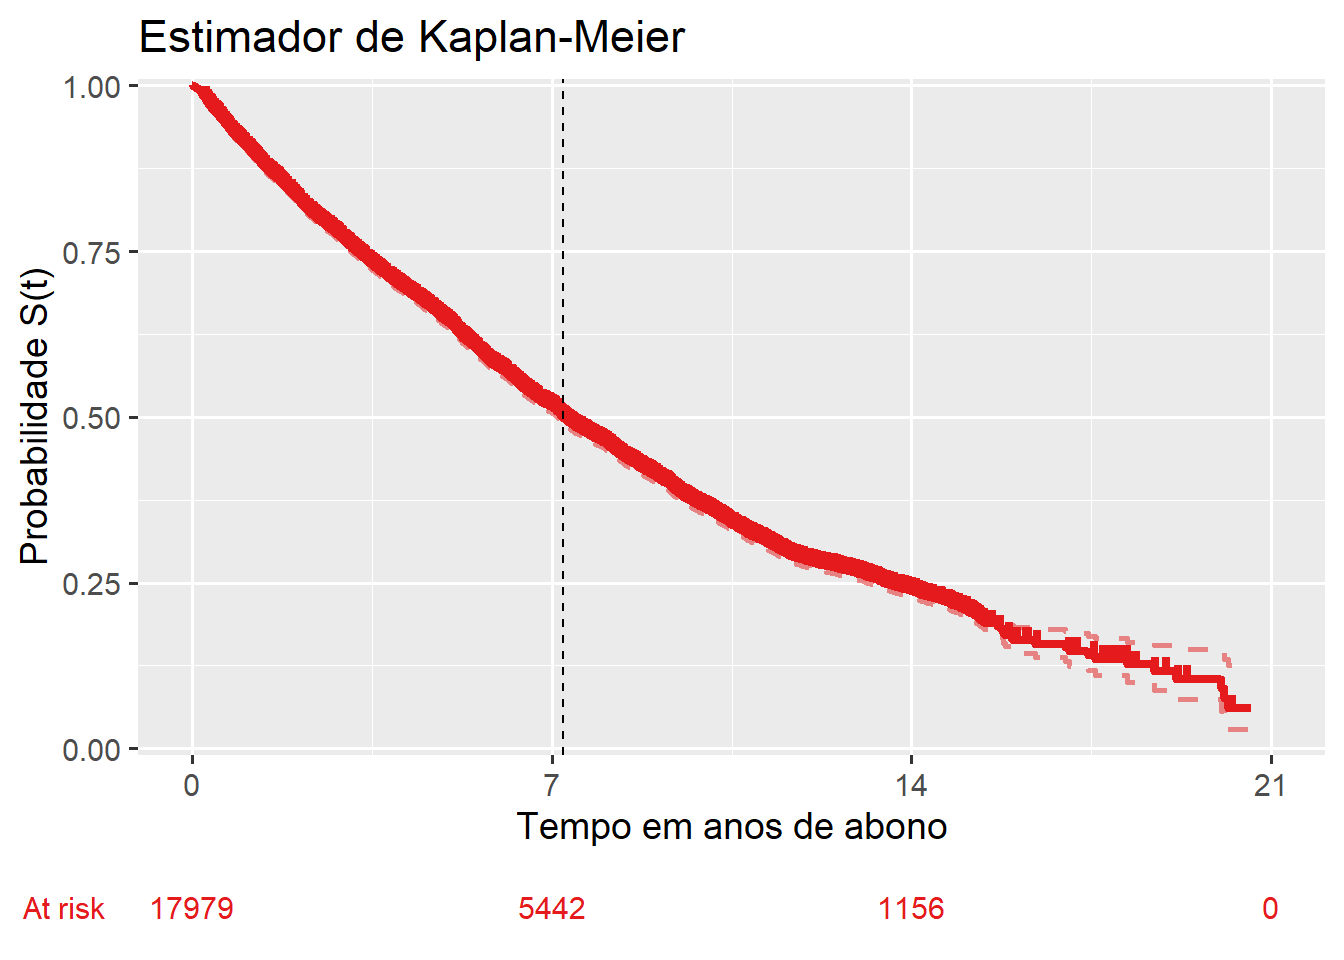
\includegraphics{Militares_Raca_files/figure-latex/unnamed-chunk-4-1.pdf}

\begin{Shaded}
\begin{Highlighting}[]
\KeywordTok{rm}\NormalTok{(.df, .plot)}
\end{Highlighting}
\end{Shaded}

\#\texttt{\{r\}\ require("ggplot2")\ .df\ \textless{}-\ data.frame(x\ =\ militares\$QUADRO,\ z\ =\ militares\$RACA,\ s\ =\ militares\$POSTO\_GRADUACAO)\ .df\ \textless{}-\ as.data.frame(with(.df,\ prop.table(table(x,\ z,\ s),\ margin\ =\ 3)))\ .plot\ \textless{}-\ ggplot(data\ =\ .df,\ aes(x\ =\ x,\ y\ =\ Freq,\ fill\ =\ z))\ +\ geom\_bar(width\ =\ 0.9,\ \ \ \ \ \ position\ =\ "fill",\ stat\ =\ "identity")\ +\ scale\_fill\_brewer(palette\ =\ "Blues")\ +\ \ \ \ \ \ scale\_y\_continuous(expand\ =\ c(0.01,\ 0),\ labels\ =\ scales::percent\_format())\ +\ \ \ \ \ \ facet\_wrap(\textasciitilde{}s)\ +\ xlab("QUADRO")\ +\ ylab("Percent")\ +\ labs(fill\ =\ "RACA")\ +\ theme\_grey(base\_size\ =\ 6,\ \ \ \ \ \ base\_family\ =\ "sans")\ +\ theme(panel.spacing\ =\ unit(0.3,\ "lines"),\ legend.position\ =\ "right")\ print(.plot)\ rm(.df,\ .plot)}

\end{document}
